% =========================================================================== %

\begin{frame}[t,plain]
\titlepage
\end{frame}

% =========================================================================== %

\begin{frame}{Scope For Today}
%
\begin{itemize}
\item DocStrings
	\begin{itemize}
	\item Triple Quote Strings
	\item JavaDocs and Doxygen
	\item A few cautionary words
	\end{itemize}
\item Type Hints
	\begin{itemize}
	\item What they are and what they do
	\item Linters
	\item Docstrings, Type Hints and Decorators
	\end{itemize}
\item Abstract Base Classes
	\begin{itemize}
	\item Concept
	\item Python's \texttt{abc} module and \texttt{ABC} class
	\item Advantages of using them
	\end{itemize}
\item UML Diagrams
\end{itemize}
%
\end{frame}

% =========================================================================== %

\begin{frame}{Commented}
%
\begin{center}
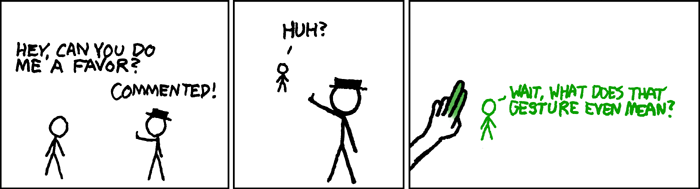
\includegraphics[width=.8\linewidth]{./gfx/15-xkcd-commented}

\vspace{12pt}
\emph{Your IDE's color may vary.}

\vspace{12pt}
Source: \url{https://xkcd.com/156/}
\end{center}
%
\end{frame}

% =========================================================================== %

\begin{frame}[fragile]{Docstrings -- \inPy{__doc__}}
%
\vspace{-3pt}
\begin{itemize}
\item All functions, classes and packages have an attribute \inPy{__doc__}
\item Contain's online help-text for any object
	\begin{itemize}
	\item Type \inPy{help(some_object)} in the REPL$^{*)}$ to see the text
	\item Or access it via \inPy{some_object.__doc__} 
	\item Lookup also works via instances: \texttt{help([])} shows help for type \inPy{list} ...
	\item ... unless the instance itself has a \inPy{__doc__} attribute.
	\end{itemize}
\item Syntax element: triple quoted strings (\inPy{"""foo bar"""})
	\begin{itemize}
	\item Contain multi-line strings
	\item Messy to use because indentation part of the string
	\end{itemize}
\item But: used to automatically set \inPy{__doc__} 
	\begin{itemize}
	\item First non-comment line of the entity
	\end{itemize}
\end{itemize}
%
\vspace{-6pt}
\begin{hintbox}[REPL]
\footnotesize
$^{*)}$ REPL means \emph{Read-Eval-Print-Loop}, \ie a programming interface where typed lines are executed (evaluated) immediately, like the Python console.
\end{hintbox}
%
\end{frame}

% =========================================================================== %

\begin{frame}[fragile]
%
\vspace{-3pt}
\begin{codebox}[Example: Function DocString]
\begin{minted}[linenos, fontsize=\scriptsize]{python3}
def print_head(text, width = 80) :
    """
    Prints a boxed headline.
    :param text: the text to put in the box
    :param width: the width in characters of the headline
    :returns: None
    
    Example:
    >>> print_head('headline', 40)
    ########################################
    #               headline               #
    ########################################
    """
    
    formattext = "{" + f":^{width - 4}" + "}"            # e.g. "{:^36}"
    print("#" * width)
    print("# " + formattext.format(text) + " #")
    print("#" * width)

help(print_head)
\end{minted}
\end{codebox}
%
\end{frame}

% =========================================================================== %

\begin{frame}[fragile]
%
\vspace{-3pt}
\begin{codebox}[Example: Limitations of automated assignment]
\begin{minted}[linenos, fontsize=\scriptsize]{python3}
def foo():
    # first line comment is not part of docstring
    """But this will be"""    
    pass
    """Anything after the first command is not part of the docstring"""

data = []
help(data)  # shows help on list

data.__doc__ = "foo bar"
help(data)  # shows "foo bar"

long_text = """This multiline text can be
used for normal variable assignments.
The line breaks are part of the string."""

def bar():
    text = """However, if you use this in functions,
    the indentation will still be part of the string,
    which probably is not what you wanted."""
\end{minted}
\end{codebox}
%
\end{frame}

% =========================================================================== %

\begin{frame}[fragile]
%
\begin{tcbraster}[raster columns=2,
                  raster equal height,
                  nobeforeafter,
                  raster column skip=0.5cm]
\begin{codebox}[Example: Class DocString]
\begin{minted}[fontsize=\scriptsize, linenos]{python3}
class Master :
    """ A masterfully created
        piece of code! """
    
    def __init__(self) :
        """ instantiates a new
            piece of baffling
            awesome software """
        print("master created")
    
    ...
\end{minted}
\end{codebox}
%
\begin{cmdbox}[Output: \texttt{help(Master)}]
\begin{minted}[fontsize=\scriptsize]{text}
class Master(builtins.object)
 |  A masterfully created piece of code!
 |  
 |  Methods defined here:
 |  
 |  __init__(self)
 |      instantiates a new piece of
 |      baffling awesome software
 |  
 |  -------------------------------------
 |  Data descriptors defined here:
 |  
 |  __dict__
 |      dictionary for instance variables
 |     (if defined)
 |  
 |  __weakref__
 |      list of weak references to the
 |      object (if defined)
\end{minted}
\end{cmdbox}
\end{tcbraster}
%
\end{frame}

% =========================================================================== %

\begin{frame}[fragile]
%
\begin{codebox}[Example: Module DocString: TextTools.py]
\begin{minted}[linenos, fontsize=\scriptsize]{python3}
""" 
Text Tools

This module offers helper tools for putting nice text on terminal outputs
"""

def print_head(text, width = 80):
    ...

def print_decobar(width = 80):
    ...
\end{minted}
\end{codebox}
%
\begin{codebox}[Example: Module Docstring: main.py]
\begin{minted}[linenos, fontsize=\scriptsize]{python3}
import TextTools

help(TextTools)
\end{minted}
\end{codebox}
%
\end{frame}

% =========================================================================== %

\begin{frame}{How Is This Better Than Comments?}
%
\begin{columns}[T]
\column{.3\linewidth}
\begin{itemize}
\item Available \enquote{on demand} (without browsing the source)
	\begin{itemize}
	\item Just type \inPy{help(some_class)} in the REPL
	\end{itemize}
\item Inheritance System
	\begin{itemize}
	\item Typing \inPy{help(my_list)} shows help text for \inPy{class list}
	\item Help on inherited methods shown with the derived class
	\end{itemize}
\end{itemize}
\pause
%
\column{.3\linewidth}
\begin{itemize}
\item Often IDE-Support
	\begin{itemize}
	\item Hover over function calls to see docstrings
	\item Details vary, but concept widely supported
	\end{itemize}
\end{itemize}
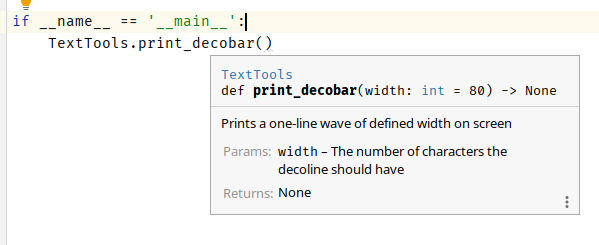
\includegraphics[width=\linewidth]{./gfx/15-helptext-mouseover}
\pause
%
\column{.3\linewidth}
\begin{itemize}
\item Two methods for inserting comments allow classification
	\begin{itemize}
	\item \enquote{Normal} comments (\texttt{\#}): explain how code \emph{works}
	\item[\Thus] Needed when you want to \emph{edit} the code
	\item Docstrings: explain how code \emph{is used}
	\item[\Thus] Needed when you want to \emph{use} the code
	\end{itemize}
\end{itemize}
\end{columns}
%
\end{frame}

% =========================================================================== %

\begin{frame}[fragile]
%
\begin{codebox}[Example: DocStrings and Comments]
\begin{minted}[linenos, fontsize=\scriptsize]{python3}
import numpy as np
def numpy_isqrt(number):
    """ approximates 1 / sqrt(number) FAST """
    
    # source: https://github.com/ajcr/ajcr.github.io/blob/
    #              master/_posts/2016-04-01-fast-inverse-square-root-python.md
    # details: https://en.wikipedia.org/wiki/Fast_inverse_square_root#Algorithm
    
    y = np.float32(number)                        # ensure y is a single precision float    
    i = y.view(np.int32)                          # typecast float -> int
    i = np.int32(0x5f3759df) - np.int32(i >> 1)   # evil bit magic, making use of:
                                                  #   log_2(1/sqrt(x)) = -1/2 log_2(x)
    y = i.view(np.float32)                        # typecast int -> float
    
    # one iteration of Newton's method to increase accuracy
    threehalfs = 1.5
    x2 = number * 0.5
    y = y * (threehalfs - (x2 * y * y))
    return float(y)
\end{minted}
\end{codebox}
%
\end{frame}

% =========================================================================== %

\begin{frame}{JavaDocs and Doxygen}
%
\begin{itemize}
\item JavaDocs: Similar Concept from Java
	\begin{itemize}
	\item On demand help in comments
	\item Special Syntax elements in comments allow automated formatting
	\item Introduced by \texttt{/**} (normal comments begin with \texttt{/*} in Java)
	\item Elements like \texttt{@param} (names a parameter and what it does)
	\end{itemize}
	\pause
\item Doxygen
	\begin{itemize}
	\item Reads structure and comments of code in various languages
	\item Parses these special commands to generate professional-looking help files
	\item HTML and PDF
	\item Doxygen for Python: uses DocStrings
	\item See \url{https://www.doxygen.nl/}
	\end{itemize}
\end{itemize}
%
\end{frame}

% =========================================================================== %

\begin{frame}{Example and Cautionary Words}
%
\begin{columns}
\column{.5\linewidth}
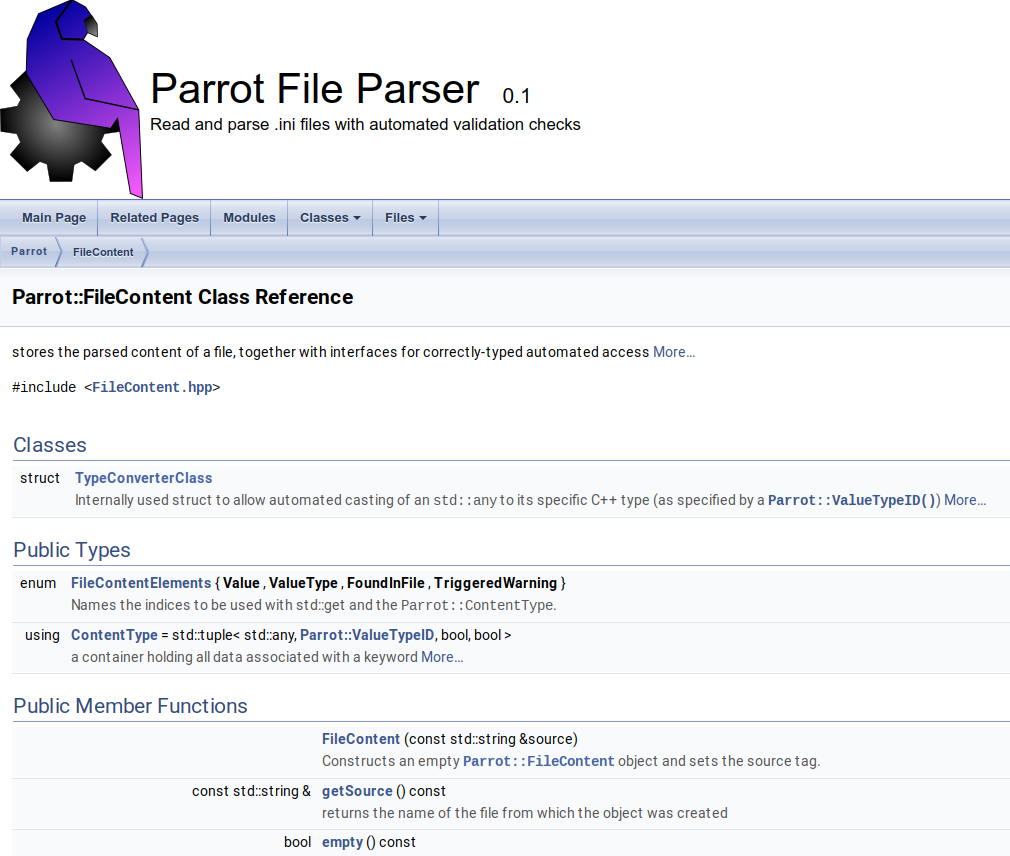
\includegraphics[width=\linewidth]{./gfx/15-parrot}
%
\column{.4\linewidth}
\begin{itemize}
\item Picture: from a (now dead) old project of mine
	\pause
\item Documentation all across code under devellopment adds a lot of noise and hinders progress
\item Good documentation is obviously good, but too much binds your ressources
	\pause
\item Tastes differ
	\begin{itemize}
	\item Current team: only in \emph{public interface}
	\item Last team: any method that does something not trivial
	\end{itemize}
\end{itemize}
\end{columns}

%
\end{frame}

% =========================================================================== %

\begin{frame}{Types}
%
\begin{columns}
\column{.6\linewidth}
\vspace{12pt}
\emph{colors.rgb(\enquote{blue}) yields \enquote{\#0000FF}. colors.rgb(\enquote{yellowish blue}) yields NaN. colors.sort() yields \enquote{rainbow}}

\vspace{12pt}
Source: \url{https://xkcd.com/1537/}
%
\column{.22\linewidth}
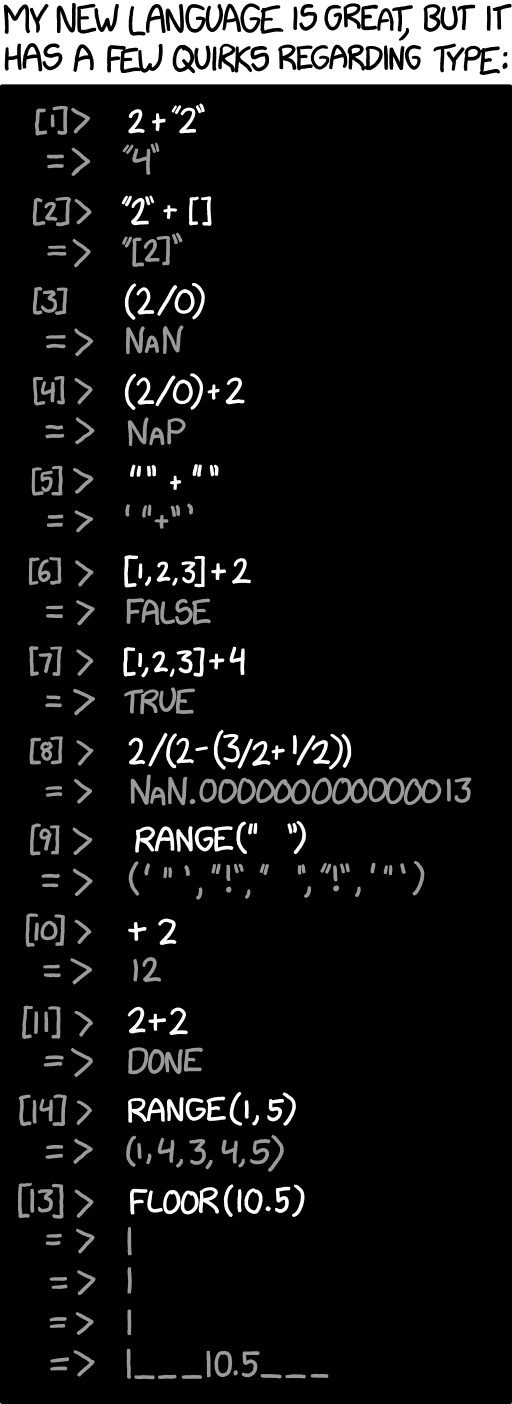
\includegraphics[width=.8\linewidth]{./gfx/15-xkcd-types}
\end{columns}
\end{frame}

% =========================================================================== %

\begin{frame}{Annotations aka Type Hints}
%
\vspace{-3pt}
\begin{itemize}
\item Python is \emph{duck typed}
	\begin{itemize}
	\item Data Type of objects can change at runtime
	\item Functions can accept any parameter as long as it's \emph{syntactically compatible}
		\begin{itemize}
		\item \inPy{a + b} will work for \inPy{int}s, \inPy{float}s, \inPy{str}ings, \inPy{list}s, ...
		\item \inPy{(a + b).capitalize()} will only work for \inPy{str}ings
		\end{itemize}
	\end{itemize}
\item Can be cool, often causes trouble
	\begin{itemize}
	\item Accidentally passing wrong data type will crash the program
	\item Not automatically detected; may happen only for specific inputs
	\item[\Thus] Hard to find and remove bugs
	\end{itemize}
\item Type hints: way to tell Python how a function is \emph{intended} to be used
\end{itemize}
%
\vspace{-6pt}
\begin{hintbox}[Namesake: \emph{Duck Typed Languages} and \emph{Duck Test}]
\footnotesize
\emph{{\color{gray}I can't prove you are a Communist.} But when I see a bird that quacks like a duck, walks like a duck, has feathers and webbed feet and associates with ducks—I'm certainly going to assume that he is a duck.}

\vspace{-18pt}
\begin{flushright}
Emil Mazey, 1946
\end{flushright}
\end{hintbox}
%
\end{frame}

% =========================================================================== %

\begin{frame}{Annotations: Syntax and What They Do}
%
\begin{itemize}
\item Syntax
	\begin{itemize}
	\item Colon + Data type after any declaration
		\begin{itemize}
		\item E.\;g. \inPy{foo: int = 42}
		\end{itemize}
	\item Return values: arrow (\texttt{->}) + Data type
		\begin{itemize}
		\item E.\;g. \inPy{def foo(bar: int) -> str}
		\end{itemize}
	\item Limiting types of containers possible by syntax \texttt{container\_type[containnee\_type]}
		\begin{itemize}
		\item E.\;g. \inPy{data: list[float]}
		\end{itemize}
	\item Type aliases possible to spare you tedious typing and communicate intent
		\begin{itemize}
		\item \inPy{Vector = list[float]} 
		\item \inPy{def dot_product(v1: Vector, v2: Vector) -> float}
		\end{itemize}
	\item Dedicated module \texttt{typing} for more involved typing logic
		\begin{itemize}
		\item E.\;g.: Either a \inPy{float} or an \inPy{int}: \inPy{typing.Union[float, int]}
		\end{itemize}
	\end{itemize}
	\pause
\item What They Do
	\begin{itemize}
	\item Nothing$^{*)}$
	\end{itemize}
\end{itemize}
%
\end{frame}

% =========================================================================== %

\begin{frame}[fragile]{$^{*)}$ What They \emph{Actually} Do}
%
\vspace{-3pt}
Type hints are ignored at runtime, but ...
\begin{itemize}
\item They do end up in another special attribute \inPy{__annotations__}
\item They are often used by IDEs
\item They are used by linters
	\begin{itemize}
	\item Linter: \emph{a tool that analyzes source code to flag programming errors, bugs, stylistic errors, and suspicious constructs} (Wikipedia)
	\item For example: mypy -- Linter for Python, written in Python
	\item Often directly built into IDEs (\zB PyCharm)
	\item We'll see how to use that in a couple of slides
	\end{itemize}
\end{itemize}
%
\vspace{-3pt}
\begin{hintbox}[Namesake: \emph{Linter}]
\footnotesize
Stephen C. Johnson, a computer scientist at Bell Labs, came up with the termin 1978 while working on the C programming language. The term \enquote{lint} was derived from lint, the name for the tiny bits of fiber and fluff shed by clothing, as the tool should act like the lint trap in a clothes dryer, detecting small errors to great effect.
\end{hintbox}
%
\end{frame}

% =========================================================================== %

\begin{frame}[fragile]
%
\begin{codebox}[Example: Annotated Code]
\begin{minted}[fontsize=\scriptsize, linenos]{python3}
import cmath
import typing

Number = typing.Union[int, float, complex]
Vector = typing.Collection[Number]

def dot_product(a: Vector, b: Vector) -> Number:
    if len(a) != len(b):
        raise AttributeError("Vectors do not have same length!")

    return sum(x * y for x, y, in zip(a, b))

def vector_length(v: Vector) -> Number:
    return cmath.sqrt(dot_product(v, v))

def return_untyped_data():
    return ['1', '2', '3']

print(vector_length.__annotations__)
\end{minted}
\end{codebox}
%
\end{frame}

% =========================================================================== %

\begin{frame}[fragile]
%
\vspace{-6pt}
\begin{codebox}[Example: Annotated Code (Continued)]
\begin{minted}[fontsize=\scriptsize, linenos, firstnumber=last]{python3}
foo = [1, 2, 3]
print(vector_length(foo))

bar: list['str'] = ['1', '2', '3']
print(vector_length(bar))

print(vector_length(return_untyped_data()))
\end{minted}
\end{codebox}
%
\vspace{-6pt}
\begin{cmdbox}[Output: Annotated Code]
\begin{minted}[fontsize=\scriptsize]{text}
{'v': typing.Collection[typing.Union[int, float, complex]], 
 'return': typing.Union[int, float, complex]}
(3.7416573867739413+0j)

Traceback (most recent call last):
  File "/home/blue-chameleon/Documents/Py_Sci/projects/07-moremeta/TypeHints.py", 
  line 24, in main
    print(vector_length(bar))
  ...
\end{minted}
\end{cmdbox}
%
\end{frame}

% =========================================================================== %

\begin{frame}[fragile]{How \texttt{mypy} Would Have Warned You}
%
\vspace{-9pt}
\begin{cmdbox}[Install mypy]
\begin{minted}[fontsize=\scriptsize]{text}
$ python3 -m pip install mypy
\end{minted}
%$
\end{cmdbox}
%
\vspace{-9pt}
\begin{cmdbox}[Invoking mypy]
\begin{minted}[fontsize=\scriptsize]{text}
$ mypy --strict TypeHints.py 
\end{minted}
%$
\end{cmdbox}
%
\vspace{-9pt}
\begin{cmdbox}[Output: Annotated Code]
\begin{minted}[fontsize=\scriptsize]{text}
TypeHints.py:16: error: Function is missing a return type annotation  [no-untyped-def]
TypeHints.py:24: error: Argument 1 to "vector_length" has incompatible type "List[str]"; 
    expected "Collection[Union[int, float, complex]]"  [arg-type]
TypeHints.py:26: error: Call to untyped function "return_untyped_data" in typed context
    [no-untyped-call]
Found 3 errors in 1 file (checked 1 source file)
\end{minted}
\end{cmdbox}
%
\end{frame}

% =========================================================================== %

\begin{frame}{How Your IDE Might Have Warned You}
%
\begin{columns}[T]
\column{.5\linewidth}
	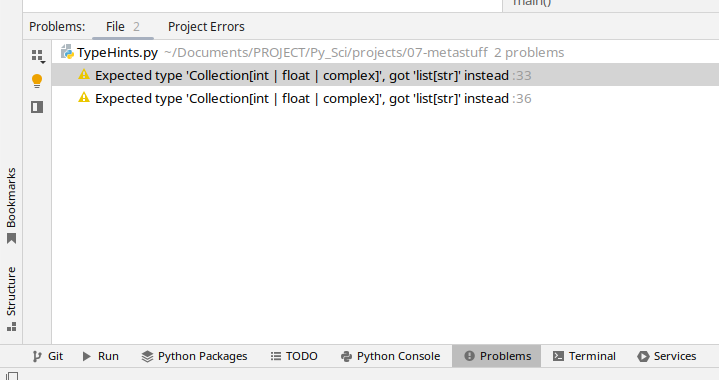
\includegraphics[width=\linewidth]{./gfx/15-pycharm-linter}
%
\column{.4\linewidth}
	\begin{itemize}
	\item Often: Problems Tab
	\item Sometimes: Squiggly lines under code, lightbulbs, etc.
	\item Sometimes: Menu \thus Code/Tools/etc \thus Check/Lint/Analyze/...
	\item Toy around, use the help, or your search engine of choice
		\begin{itemize}
		\item Search for <\emph{name of IDE}> <\emph{linter}>
		\end{itemize}
	\end{itemize}
\end{columns}
%
\end{frame}

% =========================================================================== %

\begin{frame}[fragile]
%
\begin{recapbox}[Recap: Decorators]
\footnotesize
Decorators are functions applied to other functions or classes. 
They add extra features or modify behaviour by wrapping the decorated object in another structure.

\vspace*{5pt}
There is a special syntax to apply decorators directly upon defining the object:
\begin{minted}{python3}
@decorator
def function(...):
    ...
\end{minted}
is equivalent to
\begin{minted}{python3}
def function(...):
    ...
function = decorator(function)
\end{minted}

Python packages provide many useful decorators such as \texttt{functools.cache}.

See lecture 2 for details.
\end{recapbox}
%
\end{frame}

% =========================================================================== %

\begin{frame}[fragile]{Decorators and Special Attributes}
%
\begin{itemize}
\item Problem: decorators \enquote{destroy} (\ie hide away) information of special attributes
	\begin{itemize}
	\item \inPy{foo.__name__} will give \texttt{foo}, but \inPy{decorator(foo).__name__} will give \texttt{wrapper}
	\item Likewise: \inPy{__qualname__}, \inPy{__module__}, \inPy{__annotations__} and \inPy{__doc__}
	\end{itemize}
	\pause
\item Solution (manually): copy special attributes from decorated function onto wrapper
	\pause
\item Solution (simpler): Use \texttt{functools.wraps} decorator on wrapper
%
\begin{codebox}[Scheme: Special Attribute Preserving Decorator]
\begin{minted}[fontsize=\scriptsize, linenos]{python3}
import functools

def decorator(f):
    @functools.wraps
    def wrapper(*args, **kwargs):
        ...
    return wrapper
\end{minted}
\end{codebox}
\end{itemize}
%
\end{frame}

% =========================================================================== %

\begin{frame}{Bonding}
%
\begin{columns}
\column{.4\linewidth}
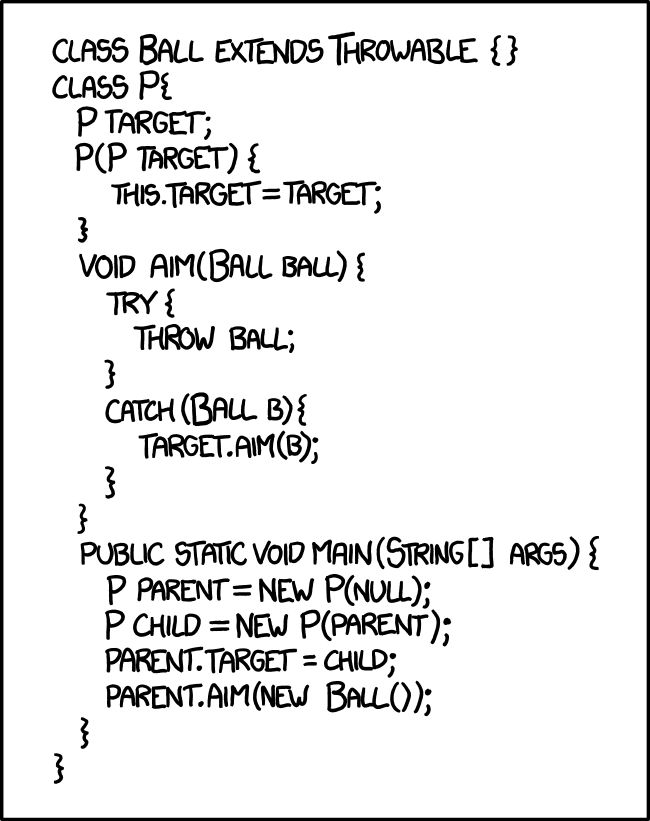
\includegraphics[width=.8\linewidth]{./gfx/15-xkcd-bonding}
%
\column{.4\linewidth}
\vspace{12pt}
\emph{I'm trying to build character but Eclipse is really confusing.}

\vspace{12pt}
Source: \url{https://xkcd.com/1188/}
\end{columns}
\end{frame}

% =========================================================================== %

\begin{frame}{Abstract Base Classes}
%
\begin{itemize}
\item Inheritance, normally:
	\begin{itemize}
	\item A \emph{base class} serves as a template for one or several derived classes.
	\item Its attributes and methods are copied onto the child class(es), unless overridden
	\end{itemize}
	\pause
\item Abstract base classes
	\begin{itemize}
	\item \enquote{Promise} methods to be present, but don't provide any implementation
	\item Only child classes that implement \emph{all} abstract methods can be instantiated
	\item Child classes that only implement \emph{some} abstract methods are abstract classes, too
	\item[\Thus] Safety mechanism: you cannot forget important features
	\end{itemize}
	\pause
\item Example: abstract class Collection
	\begin{itemize}
	\item Abstract method: \inPy{forEach(action: lambda element -> None)}
	\item Child classes \texttt{list} and \texttt{sortedset}
	\item \texttt{list}: iterates over indices
	\item \texttt{sortedset}: traverse tree structure
	\end{itemize}
\end{itemize}
%
\end{frame}

% =========================================================================== %

\begin{frame}
%
\begin{recapbox}[Metaclasses]
\footnotesize
A \emph{Metaclass} is the type of a type (\ie class).

\vspace{5pt}
Normally, \inPy{type(SomeClass) == type}, which implies certain behaviours upon instantiating the class (\ie when we type \texttt{instance = SomeClass(...)}.
We can deviate from this default behaviour by creating own metaclasses (by creating a normal class derived from \inPy{type}: \inPy{class SomeMetaClass (type): ...}).
These metaclasses then can define completely new concepts not normally present in Python.

\vspace{5pt}
To imbue new metaproperties on a self defined class, we can add \texttt{metaclass=...} to the parent classes specification:\\
\inPy{class NormalClass (ParentClass, metaclass=SomeMetaClass): ...}

This feature is rarely needed explicitly, but comes into play behind the scenes when using some packages.

\vspace{5pt}
See lecture 13 for details.
\end{recapbox}
%
\end{frame}

% =========================================================================== %

\begin{frame}{Abstract Base Classes in Python}
%
\begin{itemize}
\item Not a part of the core language features
	\pause
\item Same behaviour made available via \emph{metaclasses}
	\pause
\item No need to implement yourself
	\begin{itemize}
	\item \inPy{from abc import ABC, abstractmethod, ABCMeta}
	\item Make your class derived from \texttt{ABC} to use this language extension: \inPy{class Foo (ABC): ...}
	\item If for some reason, inheritence is not an option, you can also directly use the Metaclass: \inPy{class Foo (metaclass=ABCMeta): ...}
	\item Use the decorator \emph{@abstractmethod} to mark any method that must be overridden
	\end{itemize}
	\pause
\item Abstract Method body
	\begin{itemize}
	\item Usually empty (just use \inPy{pass})
	\item But you can still provide some shared infrastructure
	\item Derived classes can use \texttt{super().abstractMethod} to invoke this shared infrastructure.
	\end{itemize}
\end{itemize}
%
\end{frame}

% =========================================================================== %

\begin{frame}[fragile]
%
\vspace{-3pt}
\begin{codebox}[Instantiating ABCs]
\begin{minted}[linenos, fontsize=\scriptsize]{python3}
from abc import ABC, abstractmethod

class Abstract(ABC):
    @abstractmethod
    def foo(self):
        print("foo-ing around")

class Foo(Abstract):
    pass

class Bar(Abstract):
    def foo(self):
        super().foo()
        print("I'm in a Bar.")

# a = Abstract()  -- TypeError: Can't instantiate abstract class Abstract 
#                               with abstract method foo
# f = Foo()       -- dito
b = Bar()
b.foo()           ## shows "foo-ing around" and "I'm in a Bar."
\end{minted}
\end{codebox}
%
\end{frame}

% =========================================================================== %

\begin{frame}{Why would I want that?}
%
\begin{itemize}
\item Early failure reveals difficult to find bugs
	\begin{itemize}
	\item Better fail to create instance than to only detect crash when trying out a specific feature that you might forget to test
	\item Works well together with Type Hints/Linters
	\end{itemize}
	\pause
\item Separate Intent from Implementation
	\begin{itemize}
	\item Intent: operate on some \emph{collection of values} \Thus \inPy{class Collection(ABC)}
		\begin{itemize}
		\item E.\;g. write them to a file, find the biggest one, ...
		\end{itemize}
	\item Implementation: \inPy{list}, \inPy{set}, \inPy{frozenset}, ...
	\item[\Thus] Adds flexibility: you can pass any \texttt{Collection} into your method
	\item[\Thus] Decouples your method from implementation details
		\begin{itemize}
		\item Is index access available?
		\item What is the fastest way of [achieving the goal the abstract method promises]?
		\end{itemize}
	\end{itemize}
	\pause
\item Good Place for Documentation
	\begin{itemize}
	\item ABCs rarely change \Thus longer texts here don't hurt much
	\item If we do look at them, it's often for guidance, anyway
	\item Inheritance of docs means they are available on the concrete classes and instances, too
	\end{itemize}
\end{itemize}
%
\end{frame}

% =========================================================================== %

\begin{frame}{Tech Support Cheat Sheet
}
%
\begin{columns}
\column{.53\linewidth}
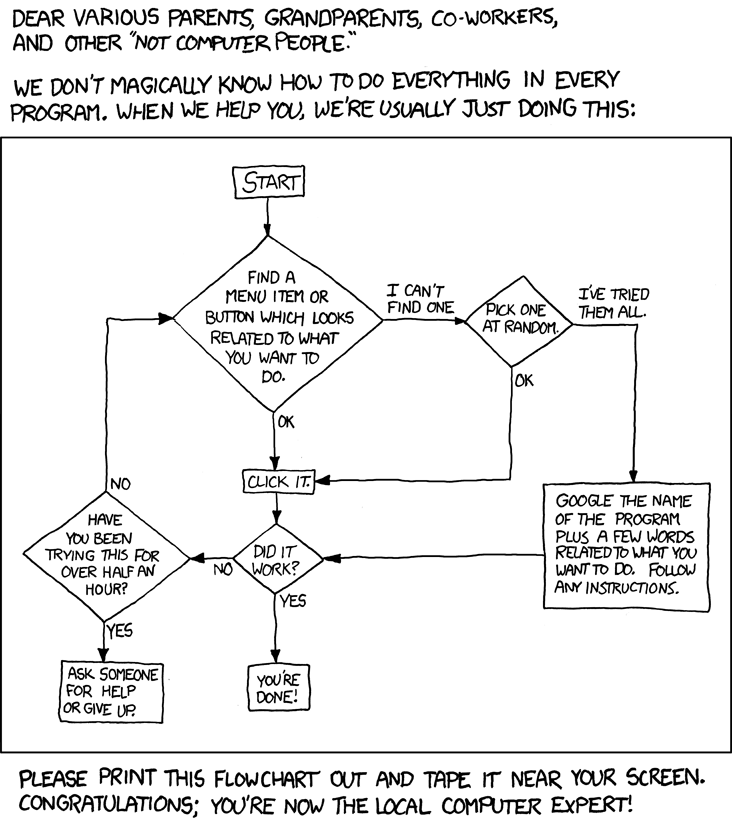
\includegraphics[width=.8\linewidth]{./gfx/15-xkcd-tech-support-cheat-sheet}
%
\column{.37\linewidth}
\vspace{12pt}
\emph{\enquote{Hey Megan, it's your father. How do I print out a flowchart?}}

\vspace{12pt}
Source: \url{https://xkcd.com/627/}
\end{columns}
\end{frame}

% =========================================================================== %

\begin{frame}{UML Diagrams}
%
\begin{itemize}
\item Unified Modeling Language
\item Family of diagrams used to visualize programming related ideas
\item Process diagrams (flowcharts), state diagrams, sequence diagrams, \textbf{class diagrams}
\item 99\% intuitive to read
\end{itemize}
%
\end{frame}

% =========================================================================== %

\begin{frame}{Class Diagrams I: Members}
%
\vspace{-6pt}
\begin{columns}
\column{.3\linewidth}
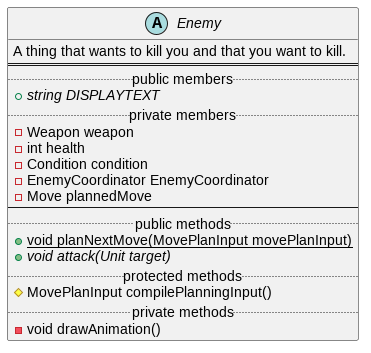
\includegraphics[width=\linewidth]{./gfx/15-uml-detail}
%
\column{.63\linewidth}
\begin{itemize}
\item Headline: Class name plus symbol for class type (abstract, enum, ...)
\item Compartments for attributes, methods and comments
\item May be subdivided (dotted lines)
\item Member (and type, though only sometimes; syntax as the language dictates it)
\item Symbols/colours encode access (public/protected/private) and type (attribute/method)
\item Underlined items: \enquote{static} members (class attributes/class methods)
\item Italics items: abstract
\end{itemize}
\end{columns}
%
\end{frame}

% =========================================================================== %

\begin{frame}{Class Diagrams II: Class Relationships}
%
\begin{columns}
\column{.5\linewidth}
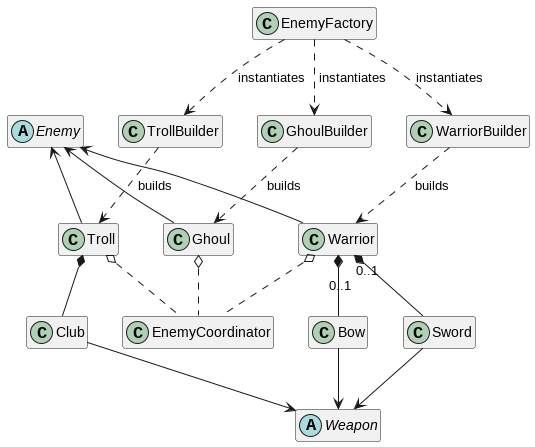
\includegraphics[width=\linewidth]{./gfx/15-uml-big}
%
\column{.4\linewidth}
\begin{itemize}
\item Arrows: Inheritance
\item Dashed lines: other relation, labelled
\item Filled Diamonds: composition (\enquote{contains} reationship)
	\begin{itemize}
	\item Sometimes with multiplicity (at least ... and up to ...)
	\end{itemize}
\item Empty Diamonds: aggregation (\enquote{uses but does not own} reationship)
\item Members or extract of members can appear (if you have enough space)
\end{itemize}
\end{columns}
%
\end{frame}

% =========================================================================== %

\begin{frame}{PlantUML}
%
\begin{itemize}
\item Free Tool for creating UML diagrams
\item Text files to PNGs
\item Available as JAR
	\begin{itemize}
	\item Requires JRE and knowledge how to run JARs:\\
		\texttt{java -jar path-to-plantuml.jar}
	\item Plugins for several code editors available, \zB Eclipse, Notepad++
	\end{itemize}
\item MIT Licence
	\begin{itemize}
	\item Open Source
	\item The MIT license gives express permission for users to reuse code for any purpose, sometimes even if code is part of proprietary software. 
	\end{itemize}
\item See \url{https://plantuml.com/}
\end{itemize}
%
\end{frame}

% =========================================================================== %